\chapter{Graphs}
%%%%%%%%%%%%%%% SECTION HEADER %%%%%%%%%%%%%%%%
\rhead{1}
\lhead{Graphs}
%%%%%%%%%%%%%%%%%%% START %%%$%%%%%%%%%%%%%%%%%
\section{Rectangle coordinate system}
The purpose of a coordinate system is to uniquely determine the position of an object on a plane.


	\begin{wrapfigure}{R}{0.3\textwidth}
		\centering
		
\includegraphics[width=0.25\textwidth]{pics/descarte.jpg}
		\caption{Portrait of Rene Descartes.}
	\end{wrapfigure}
%
\textit{Rene Descartes} devised a simple idea. He intersected two number lines at right angle and the position of a point in a plane can be determined by its distance from each of the lines. This system is called the \textbf{Cartesian coordinate system} or \textbf{rectangle coordinate system}.\\
In rectangle coordinate system, the horizontal number line called $x$-axis, and the vertical number line called $y$-axis. The origin is the intersection of the $x$- and $y$-axes. These two number lines divide, as illustrated in Figure \eqref{fig:quadrant},
the whole plane into 4 region which are called quadrant. \\
\begin{figure}[ht]
	\centering
    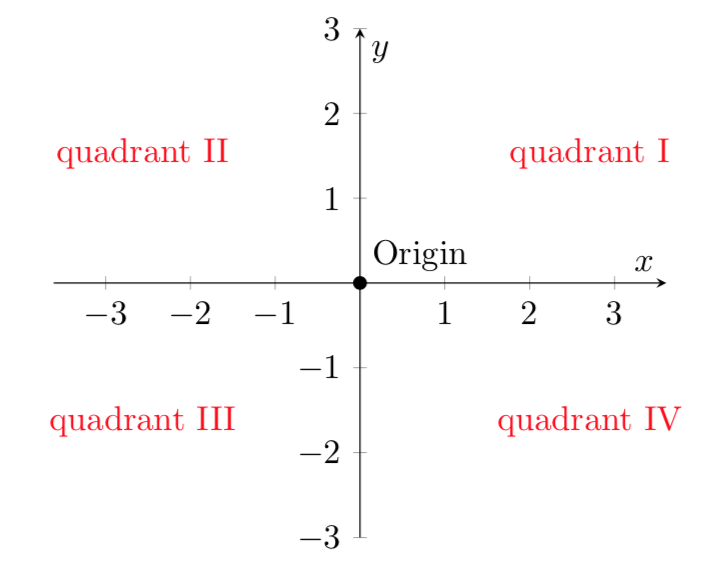
\includegraphics[width=7cm]{pics/rectangle_system.png}
    \caption{Rectangle coordinate system with its quadrants.}
    \label{fig:quadrant}
\end{figure}


Points are labeled with ordered pairs of real numbers $(x,\,y)$, called the coordinates of the point, which give the horizontal and vertical distance of the point from the origin, respectively. The origin has a ordered pair $(0,\, 0$ Locations of the points in the plane are determined in relationship to $(0,\,0)$. All points in the plane are located in one of four quadrants or on the $x$- or $y$-axis.
% ====== SECTION
\section{Plotting points}
To plot a point, start at the origin, proceed horizontally the distance and direction indicated by the $x$-coordinate, then vertically the distance and direction indicated by the $y$-coordinate. The resulting point is often labeled with its ordered pair coordinates and/or a capital letter. For example, the point $2$ units to the right of the origin and $3$ units up could be labeled $A(2,3)$.
% ======== Example 1
\begin{exa}
	Plot the following points on a rectangle coordinate system.
    $\text{A}(2, -3),\ \text{B}(0,-5),\ \text{C}(-4,1),\ \text{D}(3,0),\ \text{E}(-2,-3)$
\end{exa}
Here are the points
% 
\begin{figure}[h!tbp]
\centering
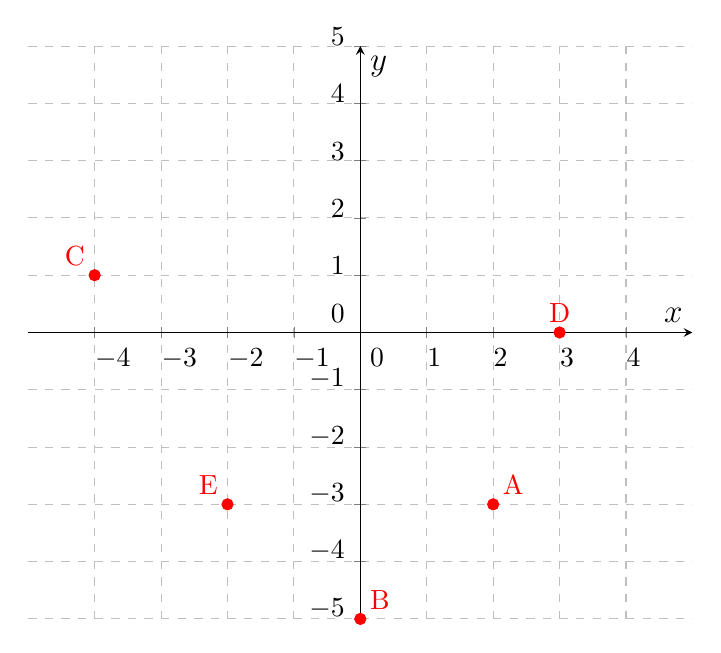
\begin{tikzpicture}
\begin{axis}[
    scale only axis,
    grid=major,
    grid style={dashed, gray!50},
    axis lines=middle,
    inner axis line style={=>},
    xlabel={\large $x$},
    ylabel={\large $y$},
    yticklabel style={inner ysep=0pt, anchor=south east},
    ytick={-5,-4,...,4,5},
    xticklabel style={inner xsep=0pt, anchor=north west},
    xtick={-4,-3,...,4},
    ymin=-5,
    ymax=5,
    xmin=-5,
    xmax=5,
    after end axis/.code={
        \path (axis cs:0,0) 
            node [anchor=north west,yshift=-0.075cm] {0}
            node [anchor=south east,xshift=-0.075cm] {0};
    }
]
    % Point A
    \addplot[mark=*,red] coordinates {(2,-3)};
    \node at (2,-3) [red, above right] {A};
    % Point B
    \addplot[mark=*,red] coordinates {(0,-5)};
    \node at (0,-5) [red, above right] {B};
    % Point C
    \addplot[mark=*,red] coordinates {(-4,1)};
    \node at (-4,1) [red, above left] {C};
    % Point D
    \addplot[mark=*,red] coordinates {(3,0)};
    \node at (3,0) [red, above] {D};
    % Point E
    \addplot[mark=*,red] coordinates {(-2,-3)};
    \node at (-2,-3) [red, above left] {E};
\end{axis}
\end{tikzpicture}
\end{figure}
% ======== SECTION
\section{Equations in two variables}
A relationship between two quantities can be expressed as an equation in two variable, such as\[
        y = 5-x^2
\]
A solution of an equation in two variables, $x$ and $y$, is an ordered pair $(x,y)$ that makes the equation a true statement. 
% ======= EXAMPLE 2
\begin{exa}
	For the linear equation $-2x+3y=8$ determine whether the ordered pair is a 
    solution.
    \begin{enumerate}[(a)]
    \item $(-4,0)$
    \item $(2,-4)$
    \item $(1, \sfrac{10}{3})$
    \end{enumerate}
\end{exa}


(a) the ordered pair $(-4,0)$ indicates that $x=-4$ and $y=0$. Substitute them into the equation:
\begin{align*}
		-2(-4)+3(0) &\stackrel{?}{=}8 \\
        8+0 & \stackrel{?}{=} 8\\
        8 &\stackrel{?}{=} 8\quad \checkmark
\end{align*}
So, $(-4,0)$ satisfies the equations and it is our solution.\\
(b) We plug $x=2$ and $y=-4$ into equation:
\begin{align*}
		-2(2)+3(-4) &\stackrel{?}{=} 8 \\
        -4-12 &\stackrel{?}{=} 8\\
        -16 &\stackrel{?}{=} 8\quad  \text{\xmark}
\end{align*}
Thus, $(2,-4)$ is not the solution.
(c) In this part, we have $x=1$ and $y=\frac{10}{3}$:
\begin{align*}
		-2(1)+3\biggl(\frac{10}{3}\biggr) &\stackrel{?}{=} 8 \\
        -2+10 &\stackrel{?}{=} 8\\
        8 &\stackrel{?}{=} 8\quad  \checkmark
\end{align*}
The ordered pair$\left(1,\frac{10}{3}\right)$ is actually one of the solution as well.
% -============
\section{Graphs of equations}
The main purpose of graphs is not to plot random points, but rather to give a picture of the solutions to an equation. We may have an equation such as $x+y=1$. We may be interested in what type of solution are possible in this equation. We can visualize the solution by making a graph of possible $x$ and $y$ combinations that make this equation a true statement.\\
We will have to start by finding possible $x$ and $y$
combinations. To find the a point on a line, just choose any number for $x$, plug it into
equation and solve for $y$. For example, to find a point on $x+y=1$, I would choose $x=0$ and I'd get $y=1$. So the ordered pair $(0,1)$ is one of many points on the line.
\begin{fact}
	You can choose a number for $x$ and solve for $y$ or vice
	versa.
\end{fact}
\begin{fact}
	Many students ask "What number should I choose?" The answer is any number! It
    is entirely up to you. But it makes sense to choose a small and simple number 
    to avoid any long and hard calculation.
\end{fact}
\vspace{0.4cm}
We'll usually draw a table, called the table of values or $xy$ table. We then choose a value, for example $x=0$ and
solve for $y$. Next, I will choose another value for $x$ and solve for $y$ again. 
\begin{center}
\begin{tabular}{ c | c }
    $x$ & $y$ \\ \hline
    \vdots	&  \vdots  \\
    0	&  ?  \\
    1   &  ?  \\
    2   &  ?  \\
    \vdots & \vdots
\end{tabular}
\end{center}
\begin{tcolorbox}[title=Steps to graph any equations,
                    fonttitle=\bfseries,
                    colframe=blue!70!red,
                    colback=white]
\begin{enumerate}[(1)]
    \item Find several ordered pairs on the equations.
    \item Plot these ordered pairs as points in the rectangle coordinate system.
    \item Connect the points with a smooth curve or line.
\end{enumerate}
\end{tcolorbox}
\begin{nt}
    In this section, we use 4 to 6 ordered pairs to graph an equation. However, you don't always need to find too many ordered pairs. Later, we will discuss how many ordered pairs we need for a specific equation.
\end{nt}
% ======= EXAMPLE 3
\begin{exa}
	Graph the equation $y=4-x$. Select integers for $x$, starting with $-3$ and ending with $3$.
\end{exa}
Our $x$ values are $-3$, $-2$, $-1$, 0, 1, 2, and 3. We plug them into the equation and solve for $y$ to find our ordered pairs.
\begin{center}
\begin{tabular}{ c | c  cl}
    $x$ & $y$ &\\
    \cline{1-2}
    $-3$	& \textcolor{red}{7}    & &$y=4-(-3)=7$ \\
    $-2$	& \textcolor{red}{6}    & &$y=4-(-2)=6$ \\
    $-1$	& \textcolor{red}{5}    & &$y=4-(-1)=5$ \\
    $0$	    & \textcolor{red}{4}    & &$y=4-(0)=4$ \\
    $1$	    & \textcolor{red}{3}    & &$y=4-(1)=3$ \\
    $2$	    & \textcolor{red}{2}    & &$y=4-(2)=2$ \\
    $3$	    & \textcolor{red}{1}    & &$y=4-(3)=1$ 
\end{tabular}
\end{center}
Next, we plot all ordered pairs and connect them to get our graph.
\begin{center}
\begin{tikzpicture}
	\begin{axis}[my style,
    minor tick num=1,
	xmin=-10, xmax=10, ymin=-10, ymax=10,
	ytick={-10,-8,-6,-4,-2,2,4,6,8,10},
	yticklabels={,-8,,-4,,,4,,8,}]
	\addplot[domain=-8:8] {4-x};
    \addplot[mark=*] coordinates {(-3,7)};
    \addplot[mark=*] coordinates {(-2,6)};
    \addplot[mark=*] coordinates {(-1,5)};
    \addplot[mark=*] coordinates {(0,4)};
    \addplot[mark=*] coordinates {(1,3)};
    \addplot[mark=*] coordinates {(2,2)};
    \addplot[mark=*] coordinates {(3,1)};
	\end{axis}
\end{tikzpicture}
\end{center}
% ===========
\begin{nt}
We can use the same method to graph an equation with absolute values. Recall that absolute values makes the inside number positive.
\end{nt}
% ====== EXAMPLE 4
\begin{exa}
    	Graph the equation $y=|x+1|$. Select integers for $x$, starting with $-4$ and ending with $2$.
\end{exa}
We begin by creating a table of values.
\begin{center}
\begin{tabular}{ c | c  cl}
    $x$ & $y$ &\\
    \cline{1-2}
    $-4$	& \textcolor{red}{3}    & &$y=|(-4)+1|=|-3|=3$ \\
    $-3$	& \textcolor{red}{2}    & &$y=|(-3)+1|=|-2|=2$ \\
    $-2$	& \textcolor{red}{1}    & &$y=|(-2)+1|=|-1|=1$ \\
    $-1$	& \textcolor{red}{0}    & &$y=|(-1)+1|=|0|=0$ \\
    $0$	    & \textcolor{red}{1}    & &$y=|(0)+1|=|1|=1$ \\
    $1$	    & \textcolor{red}{2}    & &$y=|(1)+1|=|2|=2$ \\
    $2$	    & \textcolor{red}{3}    & &$y=|(2)+1|=|3|=3$ 
\end{tabular}
\end{center}
Finally, plot all points and connect them to get the graph.
\begin{center}
\begin{tikzpicture}
	\begin{axis}[my style,
    minor tick num=1,
	xmin=-10, xmax=10, ymin=-10, ymax=10,
	ytick={-10,-8,-6,-4,-2,2,4,6,8,10},
	yticklabels={,-8,,-4,,,4,,8,}]
	\addplot[domain=-8:-1] {-x-1};
	\addplot[domain=-1:6] {x+1};
    \addplot[mark=*] coordinates {(-4,3)};
    \addplot[mark=*] coordinates {(-3,2)};
    \addplot[mark=*] coordinates {(-2,1)};
    \addplot[mark=*] coordinates {(-1,0)};
    \addplot[mark=*] coordinates {(0,1)};
    \addplot[mark=*] coordinates {(1,2)};
    \addplot[mark=*] coordinates {(2,3)};
	\end{axis}
\end{tikzpicture}
\end{center}
% ========
\subsection{\texorpdfstring{$x$}\ -intercept and \texorpdfstring{$y$}\ -intercept}
$x$-intercept and $y$-intercept are two important point on the line. The $x$-intercept is a point where a graph intersects the $x$-axis. These point are
actually the roots or zeros of an equation.\\
Whereas the $y$-intercept is a point where a graph intersects the $y$-axis. This point help us a lot and make it easier for us to graph.

\begin{figure}[ht]
	\centering
    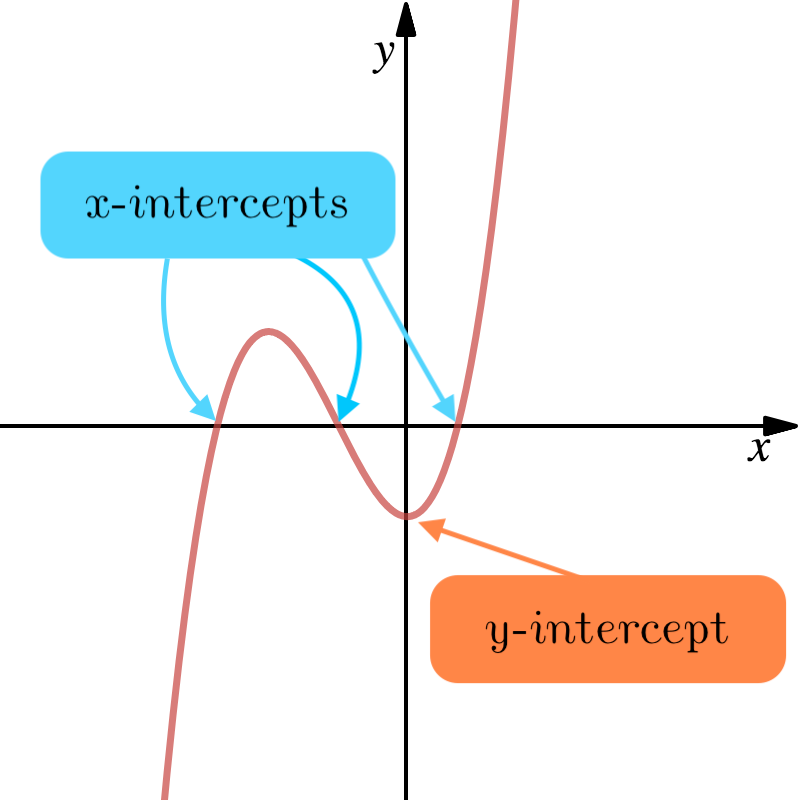
\includegraphics[width=6cm]{pics/intercept.png}
    \caption{$x$- and $y$-intercepts.}
\end{figure}

Since $x$-intercept lies on $x$-axis, therefore its $y$-coordinate is zero. 
Likewise, $y$-intercept is on $y$-axis so its $x$-coordinate is zero.
% ====== EXAMPLE 5
\newpage
\begin{exa}
    Identify the $x$- and $y$-intercepts.
\end{exa}
\noindent\begin{minipage}{0.3\textwidth}
% adapt widths of minipages to your needs
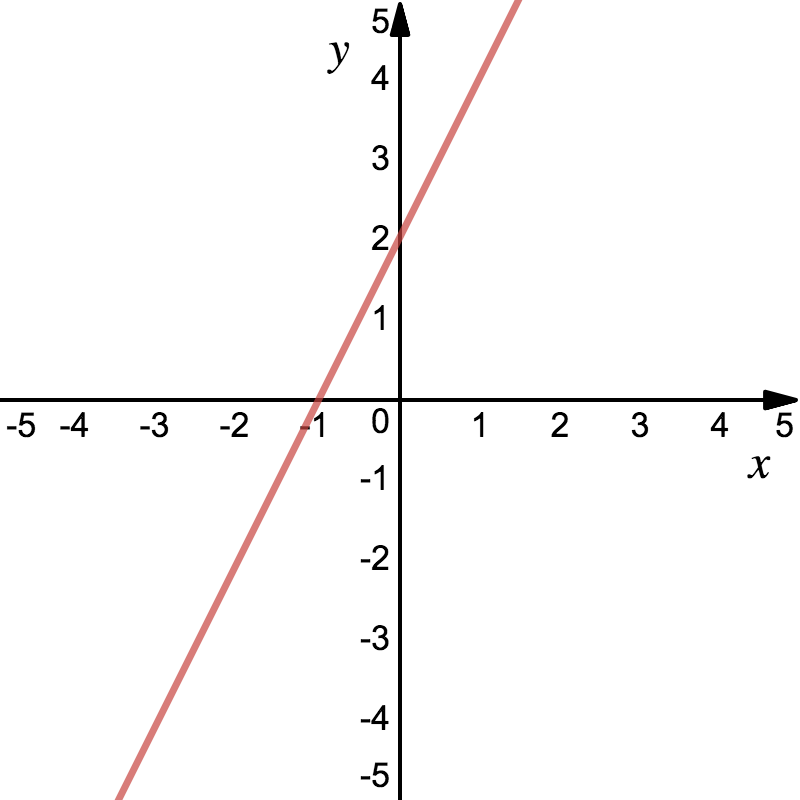
\includegraphics[width=\linewidth]{pics/ex1.png}
\end{minipage}%
\hfill%
\begin{minipage}{0.6\textwidth}
$x$-intercept: $-1$ \\
$y$-intercept: $2$
\end{minipage}


\vspace{1cm}
\begin{minipage}{0.3\textwidth}% adapt widths of minipages to your needs
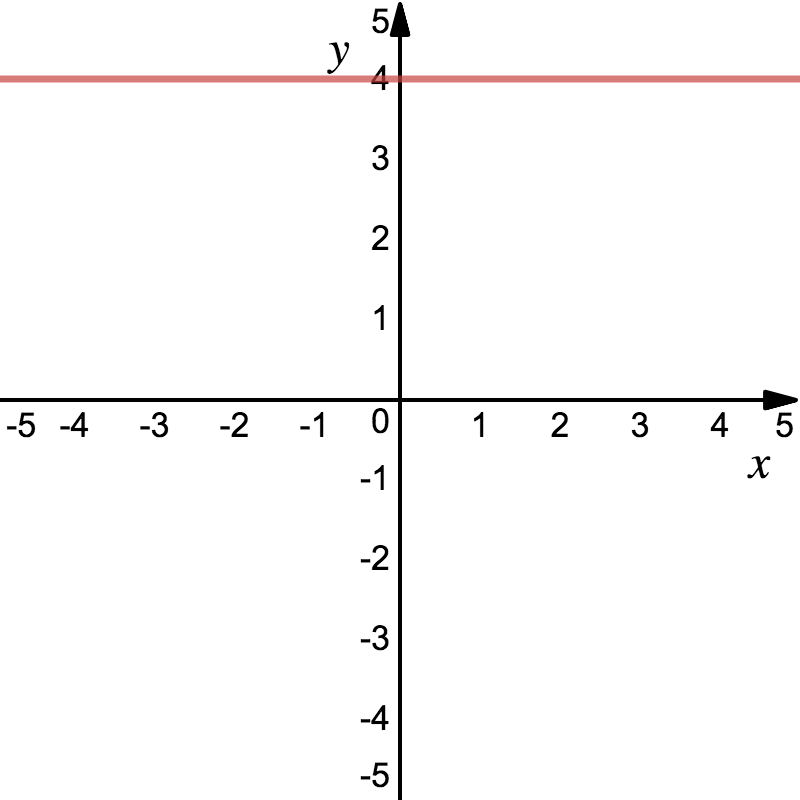
\includegraphics[width=\linewidth]{pics/ex2.png}
\end{minipage}%
\hfill%
\begin{minipage}{0.6\textwidth}
no $x$-intercept \\
$y$-intercept: $4$
\end{minipage}


\vspace{1cm}
\begin{minipage}{0.3\textwidth}% adapt widths of minipages to your needs
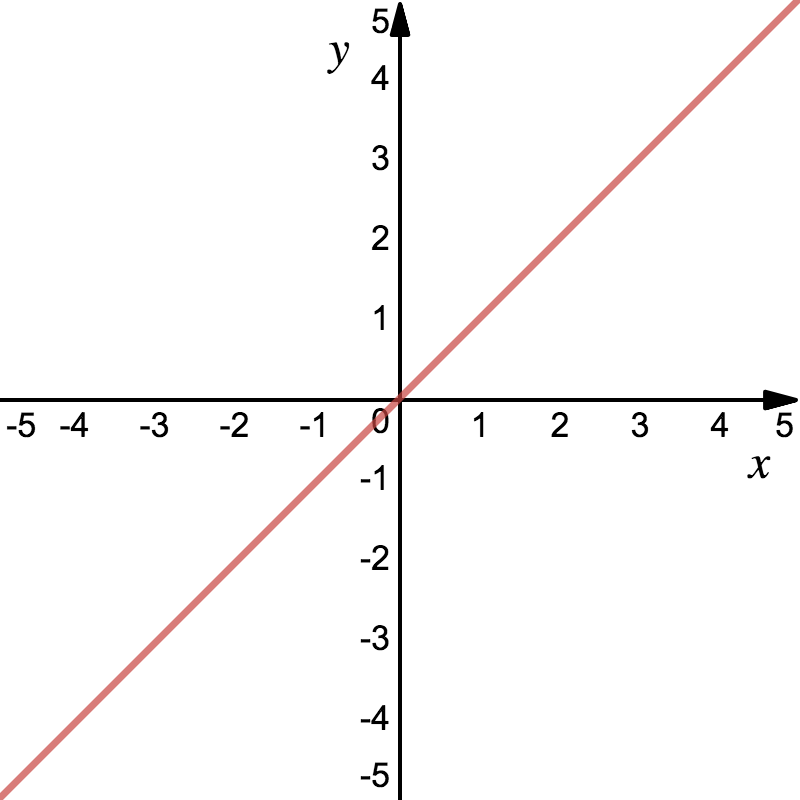
\includegraphics[width=\linewidth]{pics/ex3.png}
\end{minipage}%
\hfill%
\begin{minipage}{0.6\textwidth}
$x$-intercept: $0$ \\
$y$-intercept: $0$
\end{minipage}


\vspace{1cm}
\begin{minipage}{0.3\textwidth}% adapt widths of minipages to your needs
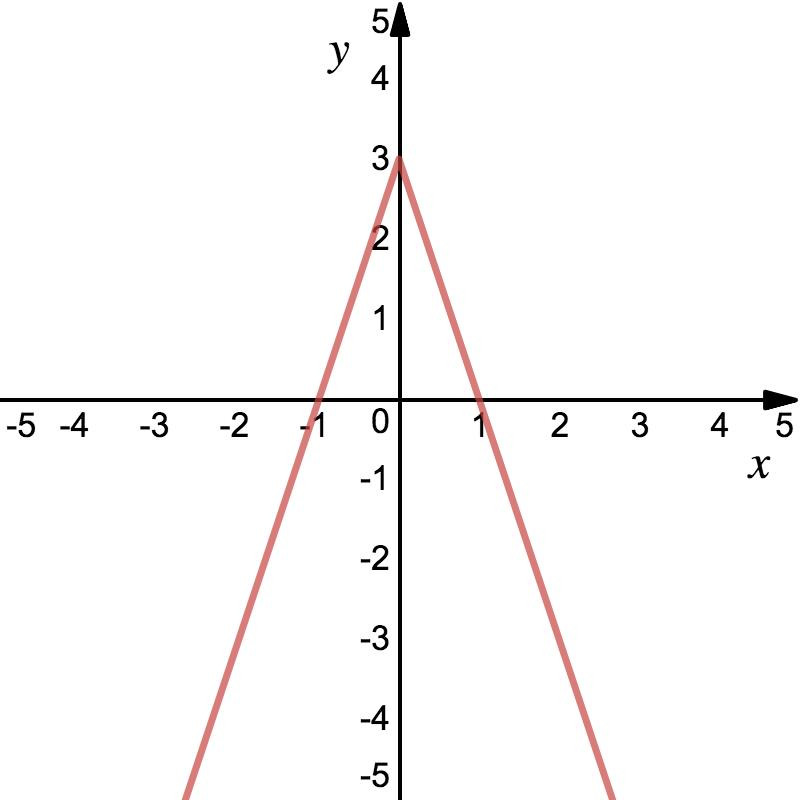
\includegraphics[width=\linewidth]{pics/ex4.png}
\end{minipage}%
\hfill%
\begin{minipage}{0.6\textwidth}
$x$-intercept: $-1$ and $1$ \\
$y$-intercept: $3$
\end{minipage}


\vspace{1cm}
\begin{minipage}{0.3\textwidth}% adapt widths of minipages to your needs
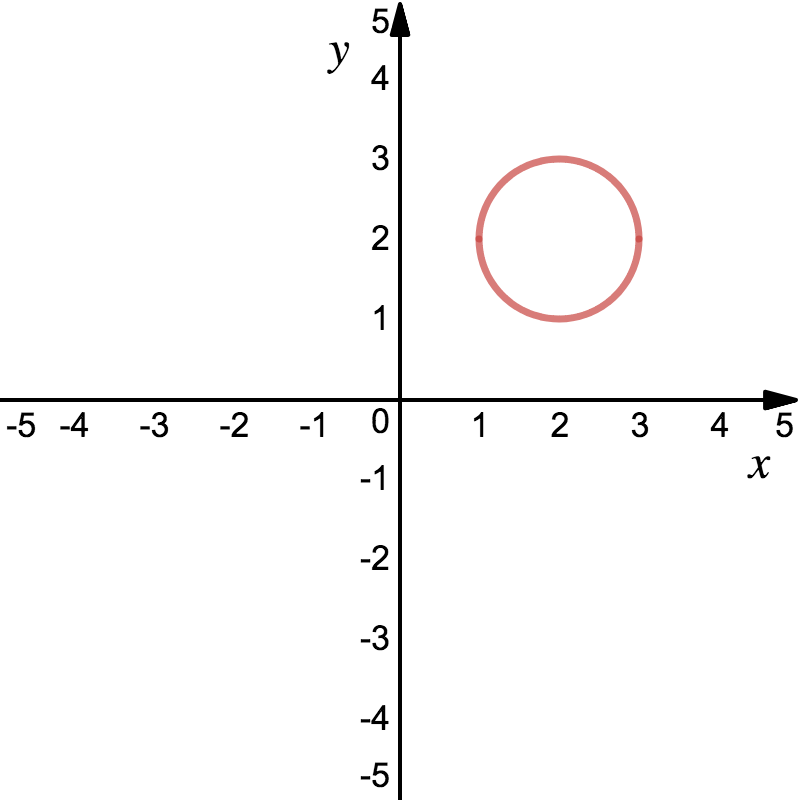
\includegraphics[width=\linewidth]{pics/ex5.png}
\end{minipage}%
\hfill%
\begin{minipage}{0.6\textwidth}
no $x$-intercept \\
no $y$-intercept
\end{minipage}

\vspace{1cm}
\begin{minipage}{0.3\textwidth}% adapt widths of minipages to your needs
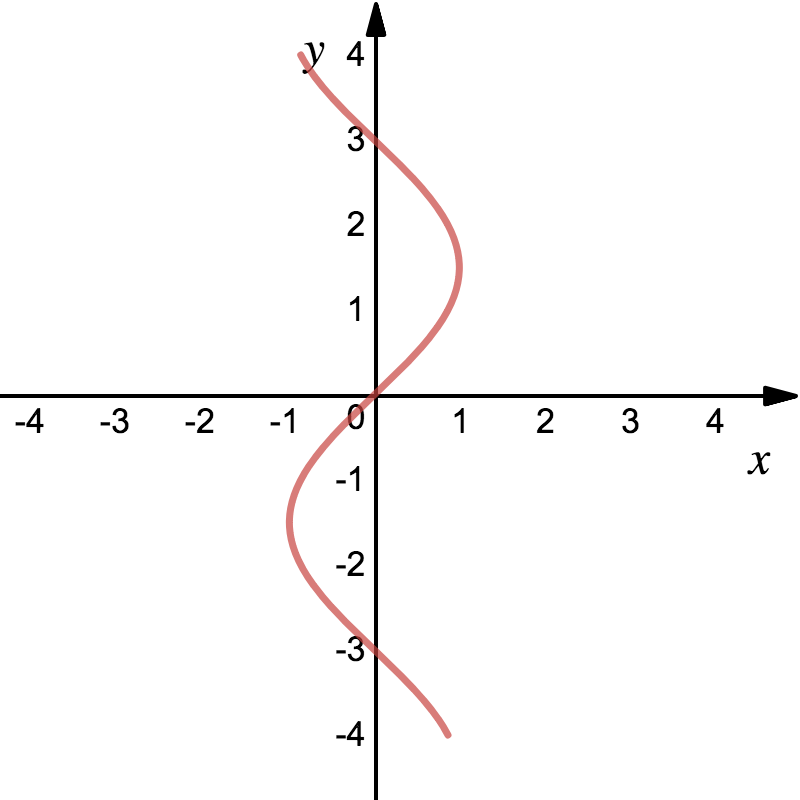
\includegraphics[width=\linewidth]{pics/ex6.png}
\end{minipage}%
\hfill%
\begin{minipage}{0.6\textwidth}
$x$-intercept: $0$ \\
$y$-intercept: $-3$, $0$ and $3$
\end{minipage}
